\begin{abstract}
In order to restore images from blurs and noise while also preserving their edges, one often applies
total variation (TV) minimization. Cauchy noise is a kind of impulsive and non-Gaussian noise whose removal can
be achieved by solving a nonconvex TV minimization problem, which is difficult due to nonconvexity and nonsmoothness. In paper \cite{MR3761275} 
a specific alternating direction method of multiplier (ADMM) is developed to solve this problem and theoretically the convergence of the method to a stationary point is established. Experimental results demonstrate that the proposed method achieves higher PSNRs for 0.5 dB average.
\end{abstract}

\section{Motivation and Outline}
Images contain natural non-Gaussian noises, such as impulse noise, Poisson noise, multiplicative noise, and Cauchy noise and may have been blurred by the point spread function (PSF) during their acquisition.
We focus on recovering images corrupted by Cauchy noise but \textbf{not} by blurring.
We assume that the original image $u$ is defined on a connected bounded domain
$\Omega \subset \R^2$ with a compacted Lipschitz boundary. The observed image with Cauchy
noise is given as

\begin{align}\label{eq:1}
    f = K u + \eta
\end{align}
with $u$ as the real, unperturbated image defined on a connected, bounded domain $\Omega \subset \mathbb{R}^2$ with a compacted Lipschitz boundary, $f\in L^2(\Omega)$ as the observation and $\eta \in L^2(\Omega)$ denoting the additive Cauchy noise. $K \in \L(L^1(\Omega),L^2(\Omega))$ representing a known linear blurring operator is set to the indicator function in the following because we don't consider blur.
The objective is to reconstruct $u$ from the observed image $f$ which is corrupted by Cauchy noise.

\section{Approach}
\subsection{Variational formulations}
\subsubsection{Convex formulation}
A convex TV-based variational method for recovering is given by
\begin{equation} \label{eq:2}
\min_{u \in BV(\Omega)} \int_\Omega \abs{{\Gdiff u}} + \frac{\lambda}{2} \left(\int_\Omega \log \left((K u - f)^2 + \gamma^2 \right) \diff x + \alpha \norm{u-\Tilde{u}}_2^2\right)
\end{equation}
with scale parameter of Cauchy distribution $\gamma > 0$ and the space of bounded TVs $BV(\Omega) = \left\{u \in L^1(\Omega) \vert TV(u) < \infty \right\}$ while the TV is defined as

\begin{equation}
    \TV(u) = \int_\Omega \abs{\Gdiff u} = \sup_{\vec{v}} \left\{ \int_\Omega u \div{\vec{v}} \diff x \, : \vec{v} \in \left(C_0^\infty(\Omega)\right)^2, \, \norm{\vec{v}}_\infty \leq 1\right\}
\end{equation}

$BV(\Omega)$ equipped with the norm $\norm{u}_{BV(\Omega)} = \norm{u}_{L^1(\Omega)} + TV(u)$ is a Banach space. The regularization parameter $\gamma > 0$ controls trade-off between TV regularization and fitting to $f$ and median filter $\Tilde{u}$, $\alpha > 0$ is a penalty parameter. The objective is \textit{strictly convex} and therefore uniquely solvable in case of $8 \alpha \gamma^2 \geq 1$. Because of \textit{strict convexity} the model \ref{eq:2} avoids issues of nonconvex optimization as the solution's dependence of numerical methods and initialization values. Due to the fact that pushing the solution $u$ to the median filter $\Tilde{u}$ does not provide satisfactory results, one unfortunately has to focus back to a \textit{nonconvex} model.
%Remember that $K(x) = \delta_x(x)$ in the variational formulations because we don't consider blur.

\subsubsection{Nonconvex formulation}
In \cite{MR3761275} an alternating direction method of multipliers (ADMM) is developed to solve the following \textit{nonconvex} variational model for denoising (and deblurring in general). Starting from any initialization the method exhibits global convergence (to a starionary point) under certain conditions. We consider

\begin{equation} \label{eq:5}
\min_{u \in BV(\Omega)} \frac{\lambda}{2} \int_\Omega \log \left((K u - f)^2 + \gamma^2 \right) \diff x + \int_\Omega \abs{{\Gdiff u}}
\end{equation}

with the regularization parameter $\gamma > 0$. While $\int_\Omega \abs{\Gdiff u}$ is \textit{convex}, due to $\log$ in the data-fitting term $\int_\Omega \left(\gamma^2 + (K u - f)^2\right) \diff x$ is \textit{nonconvex}. Therefore as already mentioned above the solution of \ref{eq:5} strongly depends of numerical method and initialization. The existence and uniqueness of solution is proven in \cite[3.2]{MR3761275}.

\subsection{ADMM Algorithm for Nonconvex and Nonsmooth Problem}
In this section the ADMM algorithmus is applied to the nonconvex variational model \ref{eq:5} recovering images degraded by Cauchy noise (and blurring in general).
Therefore we distretize the image as a set of pixels $\Omega \in \R^{n \times n}$ (mind that $n = \code{d}$ in the code) and formulate the discrete minimization nonconvex model of \ref{eq:5} by

\begin{equation}
\min_{u \in \R^{n^2}} \norm{\grad{u}{h}}_1 + \frac{\lambda}{2} \inp{\log \left(\gamma^2 \cdot \one + (K \vec{u} - \vec{f})^2 \right)}{\one}
\end{equation}

with $\one = (1,1,\ldots,1)^T \in \R^{n^2}$ being a vector of ones, $\vec{f}, \vec{u} \in \R^{n^2}$ being now vectors obtained by stacking the coloumns of the corresponding $n \times n$ images and obviously being $K = \id \in \R^{n^2 \times n^2}$ the identity matrix. $\log$ is evaluated component wise here!

While the inner product is given by $\inp{a}{b} = \sum_{i=1}^{n^2} a_i \cdot b_i$, the discretized TV regularization $\norm{\grad{u}{h}}_1$ defined as

\begin{equation}
    \TV(u) = \norm{\grad{u}{h}}_1 = \sum_{i=1}^{n^2} \sqrt{(\grad{u}{x})_i^2 + (\grad{u}{y})_i^2}
\end{equation}

with $\grad{}{x} \in \R^{n^2 \times n^2}$ and $\grad{}{y} \in \R^{n^2 \times n^2}$ being the discrete first order forward differences. The discrete gradient is defined as $\grad{u}{h} = \left[(\grad{u}{x})^T, (\grad{u}{y})^T\right]^T \in \R^{2n^2}$.

The ADMM algorithm is then derived by introducing an auxiliary variable $\vec{v} \in \R^{n^2}$ and establishing a constrained minimization problem

\begin{align}
    &\min_{u \in \R^{n^2}} \norm{\grad{u}{h}}_1 + \frac{\lambda}{2} \inp{\log \left(\gamma^2 \cdot \one + (K \vec{u} - \vec{f})^2 \right)}{\one}\\
    &\text{s.t. } Ku = v
\end{align}

Then letting $\vec{w} \in \R^{n^2}$ be the Langrangian multiplier for the constraint $Ku = v$ we obtain the corresponding augmented Lagrangian

\begin{equation}
    \mathcal{L}_{\beta}(\vec{u},\vec{v},\vec{w}) = \norm{\grad{u}{h}}_1 + \frac{\lambda}{2} \inp{\log \left(\gamma^2 \cdot \one + (K \vec{u} - \vec{f})^2 \right)}{\one} + \inp{\vec{w}}{K \vec{u}-\vec{v}} + \frac{\beta}{2} \norm{K \vec{u} - \vec{v}}_2^2
\end{equation}
with penalty parameter $\beta > 0$. This leads us directly to the algorithm for recovering the image corrupted by Cauchy noise (and in general also blurred).
See \cite[4.1]{MR3761275} for details). One obtains in total as the ADMM algorithm

\begin{enumerate}
\item INITIALIZE $\vec{u}^0$, $\vec{v}^0$, $\vec{w}^0$; set $\lambda$, $\beta$
\item For $k = 1,2,\ldots$ ITERATE $\vec{u}^{k+1}$, $\vec{v}^{k+1}$, $\vec{w}^{k+1}$ by
\begin{align}
    &\vec{u}^{k+1} \in \argmin_{\vec{u}} \norm{\grad{u}{h}}_1 + \frac{\beta}{2} \norm{K \vec{u}-\vec{v}^k+\frac{\vec{w}^k}{\beta}}_2^2 \label{eq:11}\\
    &\vec{v}^{k+1} = \argmin_{\vec{v}} \frac{\lambda}{2} \inp{\log \left(\gamma^2 \cdot \one + (\vec{v}-\vec{f})^2 \right)}{\one} + \frac{\beta}{2} \norm{K \vec{u}^{k+1} - \vec{v} + \frac{\vec{w}^k}{\beta}}_2^2 \label{eq:12}\\
    &\vec{w}^{k+1} = \vec{w}^k + \beta \left(K \vec{u}^{k+1} - \vec{v}^{k+1} \right) \label{eq:13}
\end{align}
\item STOP if $\vec{u}^{k+1}$ satisfies stopping criteria
\end{enumerate}

Convergence of the ADMM method is proved in \cite[Theorem 4.2]{MR3761275}.

Step \ref{eq:12} is solved by a Newton algorithm using the G\^ateaux derivatives of the vector valued objective $\vec{F}(\vec{v}) = \argmin_{\vec{v}} \frac{\lambda}{2} \inp{\log \left(\gamma^2 \cdot \one + (\vec{v}-\vec{f})^2 \right)}{\one} + \frac{\beta}{2} \norm{K \vec{u}^{k+1} - \vec{v} + \frac{\vec{w}^k}{\beta}}_2^2$

\begin{align}
    &\Gdiff \vec{F}(\vec{v}^k) = \lambda \frac{\vec{v}^k-\vec{f}}{\gamma^2 \cdot \one + (\vec{v}^k-\vec{f})^2} - \beta \left(\vec{u}-\vec{v}^k+\frac{\vec{w}^k}{\beta}\right) \\
    &\Gdiff^2 \vec{F}(\vec{v}^k) = \lambda \frac{\left(\gamma^2 \cdot \one + (\vec{v}^k-\vec{f})^2\right) - 2(\vec{v}^k-\vec{f})^2}{\left(\gamma^2 \cdot \one + (\vec{v}^k-\vec{f})^2\right)^2} + \beta \cdot \one = \lambda \frac{\gamma^2 \cdot \one - (\vec{v}^k-\vec{f})^2}{\left(\gamma^2 \cdot \one + (\vec{v}^k-\vec{f})^2\right)^2} + \beta \cdot \one
\end{align}

Our first approach to solve step \ref{eq:11} was using \cite{MR2049783} (see subsection \ref{subsec:chambolle}), but due to lack of convergence we used \cite{MR2722312} instead as described in the following section \ref{subsec:FGP}.

\subsection{Fast Gradient Projection (FGP)} \label{subsec:FGP}
The following method solving step \ref{eq:11} of the ADMM is described in \cite{MR2049783} and implemented in $\code{main.m}$. We use the Fast Gradient Projection method (FGP) to solve a dual problem implemented in $\code{denoising\_isotrop\_tv}$. Therefore we modified the given $\code{denoising\_anisotrop\_tv}$. In our case we restrict to the dimensions $m = n = \code{d}$.
With the isotropic TV given as

\begin{equation}
\TV_I(\vec{x}) = \sum_{i=1}^{m-1} \sum_{j=1}^{n-1} \sqrt{(x_{i,j}-x_{i+1,j})^2 + (x_{i,j} - x_{i,j+1})^2} + \sum_{i=1}^{m-1} \abs{x_{i,n} - x_{i+1,n}} + \sum_{j=1}^{n-1} \abs{x_{m,j} - x_{m,j+1}}
\end{equation}

where one assumes the standard reflexive boundary conditions $x_{m+1,j} - x_{m,j} = 0 \ \forall j$ and $x_{i,n+1} - x_{i,n} = 0 \ \forall i$.

We consider constrained minimization problems of the form
\begin{equation} \label{eq:4.1}
    \min_{\vec{x} \in C} \norm{\vec{x}-\vec{b}} + 2\lambda \TV(\vec{x})
\end{equation}
with a closed convex set $C \subset \R^{m \times n}$ with $C = B_{l,u} = \{\vec{x}: l \leq x_{ij} \leq u, \ \forall i,j\}$ where $l=0,\ u=1$.

To construct a dual of the constrained problem, we introduce the dual variables $(\vec{p},\vec{q})$ as elements of
$\mathcal{P}$ which is a set of matrix-pairs $(\vec{p},\vec{q})$ with $\vec{p} \in \R^{(m-1) \times n}$ and $\vec{q} \in \R^{m \times (n-1)}$ satisfying
\begin{align}
    p_{i,j}^2+q_{i,j}^2 &\leq 1\quad i=1,\ldots,m-1; \ j=1,\ldots,n-1\\
    \abs{p_{i,j}} &\leq 1\quad i=1,\ldots,m-1 \\
    \abs{q_{i,j}} &\leq 1\quad j=1,\ldots,n-1
\end{align}

while the entries are given by

\begin{align}
    p_{i,j} = x_{i,j} - x_{i+1,j}, \quad &i=1,\ldots,m-1; \ j=1,\ldots,n \\
    q_{i,j} = x_{i,j} - x_{i,j+1}, \quad &i=1,\ldots,m; \ j=1,\ldots,n-1
\end{align}

Furthermore the linear operator $\mathcal{L}: \R^{(m-1) \times n} \times \R^{m \times (n-1)} \mapsto \R^{m \times n}$ is defined by
\begin{equation}
    \mathcal{L}:(\vec{p},\vec{q})_{i,j} = p_{i,j} + q_{i,j} - p_{i-1,j} - q_{i,j-1} \ \forall i=1,\ldots,m; \ j=1,\ldots,n
\end{equation}

Obviously $\mathcal{L}$ is equivalent to the \textit{adjoint} discrete gradient operator $\code{G'} = (\grad{}{h})^* = -\div{}{h}$, the discrete divergence operator implemented in $\code{gradient\_discrete\_4}$.

Consequently, $\mathcal{L}^T: \R^{m \times n} \mapsto \R^{(m-1) \times n} \times \R^{m \times (n-1)}$ represents the discrete gradient operator $\code{G} = \grad{}{h}$ applying the first order forward differences in both dimensions to the stacked coloumns vector $\code{x}$. The mapping is given by

\begin{equation}
    \mathcal{L}^T(\vec{x}) = (\vec{p},\vec{q})
\end{equation}

In the code $\vec{p}$ corresponds to $\code{px}$, $\vec{q}$ coresponds to $\code{py}$ and $(\vec{p},\vec{q})$ corresponds to $\code{p1}$. Note that $\code{px}$, $\code{py}$ and $\code{p1}$ are each vectors of stacked coloumns of the image.

Next we consider the orthogonal projection operator $P_C$ on the set $C = B_{l,u}$
\begin{equation}
    P_C(\vec{x})_{ij} = P_{B_{l,u}}(\vec{x})_{ij} =
    \begin{cases}
        l &x_{ij} < l\\
        x_{ij} &l \leq x_{ij} \leq u\\
        u &x_{ij} > u
    \end{cases}
\end{equation}

In the following, we will shortly recover the Gradient Projection Method (GP) from \cite[III-B]{MR2722312}. Therefore we consider the nonsmooth convex optimization model $\min_{\vec{x}} f(\vec{x}) + g(\vec{x})$ with $g$ being a proper closed convex function and $f$ a continously Lipschitz differentiable function. The standard smooth convex constrained optimization problem $\min_{\vec{x} \in C} f(x)$ is obtained by choosing $g(\vec{x}) \equiv \delta_C$ with $C = B_{l,u} = \subset \R^{m \times n}$ being some closed convex set as above. The proximal mapping of $g = \delta_C$ is then given by $prox_t(g) = prox_t(\delta_C) = (I + t \partial \delta_C)^{-1} = P_C = P_{B_{l,u}}$ . The optimality condition for $\vec{x}^*$ solving the convex minimization problem is given by $0 \in t \grad{f}(\vec{x}) + t \partial g(\vec{x}^*)$ that is equivalent to $\vec{x}^* = (I + t \partial g)^{-1}(I - t \grad{f})(\vec{x}^*)$. This leads directly to the GP: $\vec{x}_k = P_C(\vec{x}_{k-1}-t_k \grad{f}(\vec{x}_{k-1}))$.

Coming back to the solving strategy for \ref{eq:4.1}, we further need to introduce another projection operator $P_{\mathcal{P}}$ on $\mathcal{P}$ given by
\begin{equation}
    P_\mathcal{P}(\vec{p},\vec{q)}=(\vec{r},\vec{s})
\end{equation}
where $\vec{r} \in \R^{(m-1) \times n}$ and $\vec{s} \in \R^{m \times (n-1)}$ are given by
\begin{align}
    r_{ij} = \begin{cases}
                \frac{p_{ij}}{\max\{1,\sqrt{p_{ij}^2+q_{ij}^2}\}} &i=1,\ldots,m-1; \ j=1,\ldots,n-1\\
                \frac{p_{in}}{\max\{1,\abs{p_{in}\}}} &i=1,\ldots,m-1
            \end{cases}\\
    s_{ij} = \begin{cases}
                \frac{q_{ij}}{\max\{1,\sqrt{p_{ij}^2+q_{ij}^2}\}} &i=1,\ldots,m-1; \ j=1,\ldots,n-1\\
                \frac{q_{mj}}{\max\{1,\abs{q_{mj}\}}} &j=1,\ldots,n-1
            \end{cases}
\end{align}

$(\vec{r},\vec{s})$ corresponds to $\code{r}$ in the code.

While \cite[Proposition 4.1]{MR2722312} establishes the dual problem that is convex and contains a continously differentiable objective, \cite[Lemma 4.1]{MR2722312} derives the gradient of the objective. We gain the \textbf{Fast Gradient Projection} algorithm $\textbf{FGP}(b,\lambda,N)$ given by

\begin{itemize}
    \item INPUT: $\vec{b}$ (observed image), $\lambda)$ (regularization parameter), $N$ (iterations)
    \item OUTPUT: optimal solution $\vec{x}^*$ of \ref{eq:4.1}
    \item STEP $0$: $(\vec{r}_1,\vec{s}_1) = (\vec{p}_0,\vec{q}_0) = (\vec{0}_{(m-1) \times n}, \vec{0}_{m \times (n-1)})$, $t_1 = 1$
    \item STEP $k$ ($k=1,\ldots,N$) compute
    \begin{align}
        &(\vec{p}_k, \vec{q}_k) = P_{\mathcal{P}} \left[(\vec{r}_k,\vec{s}_k) + \frac{1}{8 \lambda} \mathcal{L}^T(P_C[\vec{b}-\lambda \mathcal{L}(\vec{r}_k,\vec{s}_k)])\right]\\
        &t_{k+1} = \frac{1+\sqrt{1+4 t_k^2}}{2}\\
        &(\vec{r}_{k+1},\vec{s}_{k+1}) = (\vec{p}_k,\vec{q}_k) + \frac{t_k-1}{t_{k+1}}(\vec{p}_k-\vec{p}_{k-1},\vec{q}_k-\vec{q}_{k-1})
    \end{align}
    \item SET
    \begin{equation}
        \vec{x}^* = P_C\left[\vec{b}-\lambda \mathcal{L}(\vec{p}_N,\vec{q}_N)\right]
    \end{equation}
\end{itemize}

The FGP method works pretty fine for our applications.
The rate of convergence of the FGP measures $O(1/k^2)$.

\subsubsection{Failed approach (Chambolle)} \label{subsec:chambolle}
In this section we will shortly review our failed approach to solve step \ref{eq:11} of the ADMM with the Chambolle algorithm \cite{MR2049783} instead of FGP. This is implemented in $\code{mainChambolle.m}$, the algorithm does \textbf{not} show convergency.

Given the minimization problem where we regard $g = v^k + \frac{w^k}{\beta}$ from the ADMM
\begin{equation}
    \min_{u \in X} \frac{\norm{u-g}^2}{2 \lambda} + J(u)
\end{equation}
one gets that $w = (g-u)/ \lambda$ is the minimizer of
\begin{equation}
    \frac{\norm{w-(g/ \lambda)}^2}{2} + \frac{1}{\lambda} J^*(w)
\end{equation}
where $J*=\chi_K$ of a convex set $K$. One deduces $w = \pi_K(g/ \lambda)$, hence the minimizing $u$ is given as $u = g-\pi_{\lambda K}(g)$. Computing $\pi_{\gamma K}(g)$ amounts to solving the problem

\begin{equation}
    \min \left\{ \norm{\lambda \div p -g}^2: \ p \in Y, \ \abs{p_{ij}}^2 -1 \leq 0 \ \forall i,j = 1,\ldots,N \right\}
\end{equation}

Using Karush-Kuhn-Tucker conditions and a Lagrange multiplier this leads to the fixed point iteration

\begin{equation}
    p_{i,j}^{n+1} = \frac{p_{i,j}^n + \tau(\grad(\div p^n - g/ \lambda))_{i,j}}{1+\tau \abs{(\div p^n - g/ \lambda))_{i,j}}}
\end{equation}

\cite[Theorem 3.1]{MR2049783} shows that $\lambda \div p^n$ converges to $\pi_{\lambda K}(g)$ for $n \to \infty$.

Since $\sigma$ is less difficult to determine than $\lambda$, we proposed another algorithm that tackles directly the solution of the objective

\begin{equation} \label{eq:Ch11}
    \min \left\{ J(u): \norm{u-g}^2 = N^2 \sigma^2 \right\}
\end{equation}
The task is to find $\lambda > 0$ s.t. $\norm{\pi_{\lambda K} g}^2 = N^2 \sigma^2$. Set $f(s) = \norm{\pi_{sK}g}$.

Then the following algorithm was supposed to solve \ref{eq:Ch11}. The goal is to find $\overline{\lambda} > 0$ s.t. $f(\overline{\lambda}) = \norm{\pi_{\overline{\lambda}K}g} = N \sigma$.
\begin{itemize}
    \item assume $N \sigma \in [0, \norm{g-<g>}]$
    \item set $\lambda_0 > 0$
    \item set $v_0 = \pi_{\lambda_0 K}(g) (=\lambda_0 \div p)$
    \item set $f_0 = f(\lambda_0) = \norm{v_0}$
    \item step $\lambda_{n+1} = \frac{N \sigma}{f_n} \lambda_n$
    \item step $v_{n+1} = \pi_{\lambda_{n+1}K}(g) = \lambda_{n+1} \div p$
    \item step $f_{n+1} = \norm{v_{n+1}}$
\end{itemize}

\cite[Theorem 4.2]{MR2049783} proofs that for $n \to \infty$, $f_n \to N \sigma$ the expression $g-v_n$ converges to the unique solution of \ref{eq:Ch11}.\\

Our assumption was that the update of $\lambda = 1/ \beta$ ($\beta$ from ADMM) in each step of the $\code{tv\_MinimizationChambolle}$ might cause the problem of non-existing convergence in the implementation, but skipping the substep did not change anything.

\section{Experiments and results}
In accordance to \cite{MR3761275} we used the peak signal to noise ratio (PSNR) and the structured similarity index (SSIM) as measures for the performance of the algorithm. The PSNR shows better performance as it becomes larger whereas the SSIM shows better performance as it approaches 1. The following two images depict the history of SSIM and PSNR for the third color channel over all iterations, together with the resulting image for some parameter settings.\\
The parameters in question are $\gamma$, $\beta$ and $\lambda$ as defined in \cite{MR3761275}. $\gamma$ corresponds to the scale parameter of the Cauchy distribution used to degrade the image. Throughout all tests we set $\gamma=0.1$ which results in noisy images as depicted in figure \ref{fig2} and figure \ref{fig3}.\\
\begin{figure}[H]
    \centering
    \begin{minipage}[b]{0.45\textwidth}
    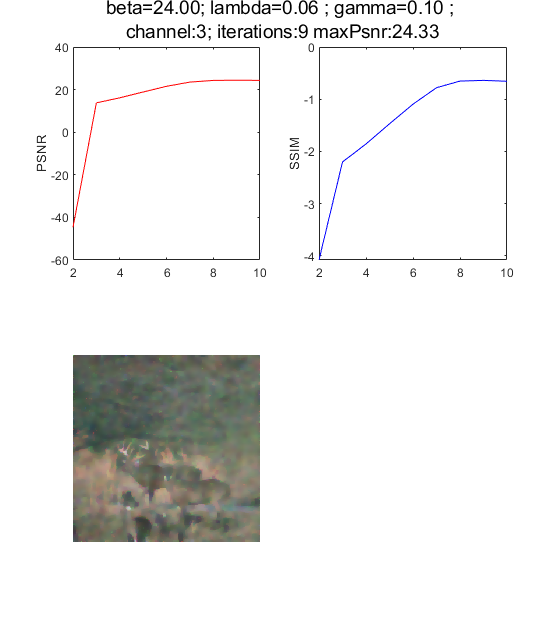
\includegraphics[scale=0.6]{images/statTest3.png}
    \end{minipage}
    \hfill
    \begin{minipage}[b]{0.45\textwidth}
    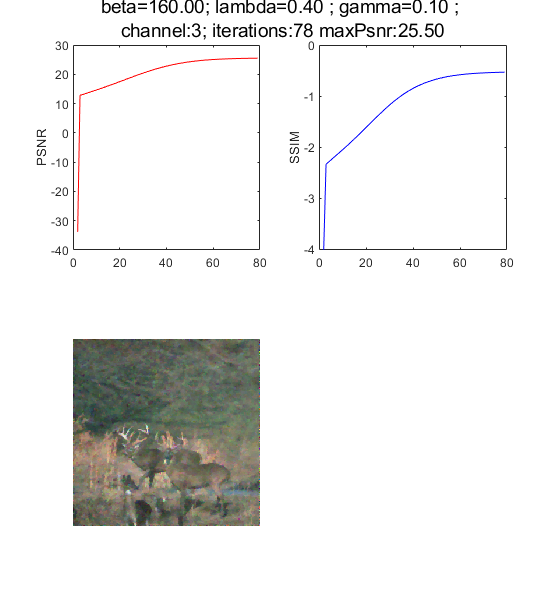
\includegraphics[scale=0.6]{images/statTest1.png}
    \end{minipage}
    \caption{Result of two setups with different parameter settings}
    \label{fig1}
\end{figure}
\vspace{1cm}
$\lambda$ is the weight for the data term in our objective function and $\beta$ is the weight for the relaxed constrained of the auxiliary variable $v$. Therefore, increasing $\lambda$ and/or $\beta$ induces less weight on the TV regularization which aims for sharper images but might not filter out noise efficiently.\\
Figure \ref{fig1} compares the result of two parameter setups. In the first setting $\lambda$ and $\beta$ are rather small whereas in the second setting they take larger values. There is no great difference in the achieved PSNR however the setting with larger parameter values is indeed more blurry than the other setup which also does not seem to still contain much noise.$\lambda$ and $\beta$ also affect the number of total iterations of the algorithm in the way, that larger values infer more iterations.

\begin{figure}[H]
    \centering
    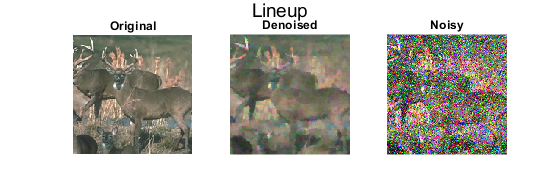
\includegraphics[scale=1]{images/test1.png}
    \caption{Comparison of result in right figure in \ref{fig1} vs true and degraded image (zoomed in)}
    \label{fig2}
\end{figure}
\vspace{2cm}
Figure \ref{fig3} shows the results for the primal dual algorithm for the anisotropic TV as described in \cite{MR2722312}, solving the problem
\begin{align}
   \argmin_{\vec{u}} \lambda \norm{\grad{u}{h}}_1 + \frac{\norm{u-f}^2}{2}
\end{align}
Which is the classical objective for TV regularization, paired with a data term. We let the algorithm iterate for 200 iterations. The denoised image still contains a lot of noise while it is also quite blurry. This is mirrored also in the PSNR value which is considerably lower than the values achieved by the proposed ADMM.

\begin{figure}[H]
    \centering
    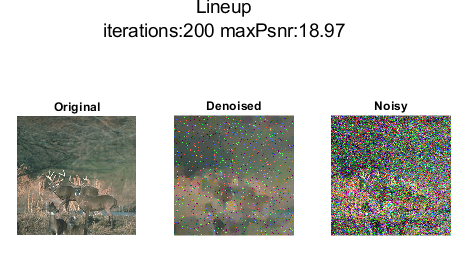
\includegraphics[scale=1]{images/onlyAnisoTv.png}
    \caption{In this setting we applied the primal dual algorithm in \cite{MR2722312} for anisotropic TV denoising to the objective function $\lambda \norm{\grad{u}{h}}_1 + \frac{\norm{u-f}^2}{2}$}
    \label{fig3}
\end{figure}
Table \ref{tab:table1} shows some PSNR results, together with the number of iterations needed to achieve them. It strikes that better results always need more iterations to reach their maximal PSNR value.
\begin{table}[h!]
  \begin{center}
    \label{tab:table1}
    \begin{tabular}{|l|l|l|l|l|l|l|l|}
      \hline
      $\beta$ & 4 & 40 & 50 & 20 & 100 & 140 & 160\\
      \hline
      $\lambda$ & 0.01 & 0.1 & 0.5 & 0.01 & 0.2 & 0.2 & 0.4\\
      \hline
      PSNR & 23.42 & 24.51 & 24.35 & 23.75 & 25.08 & 25.1 & \textbf{25.4}\\
      \hline
      iterations & 10 & 14 & 46 & 8 & 32 & 42 & 78\\
      \hline
    \end{tabular}
    \caption{Results for various parameter settings}
  \end{center}
\end{table}

\section{Conclusion}
The proposed method proves to perform quite well on the stated problem. We did not actually address an image model as 
\begin{align}%\label{eq:1}
    f = Ku + \eta
\end{align}
but rather as
\begin{align}%\label{eq:1}
    f = u + \eta
\end{align}
since in \cite{MR3761275} the method in \cite{MR2049783} was used to solve the sub problem \ref{eq:11}, but in \cite{MR2049783} it is explicitely stated, that the involvement of $K$ is a different problem to which, so far, they did not find a solution.